\documentclass[spanish,12pt,a4paper,titlepage]{report}
\usepackage[utf8]{inputenc}
\usepackage{graphicx}
\usepackage{subfig}
\usepackage{float}
\usepackage{wrapfig}
\usepackage{multirow}
\usepackage{caption}
\usepackage[spanish]{babel}
\usepackage[dvips]{hyperref}
\usepackage{amssymb}
\usepackage{listings}
\usepackage{epsfig}
\usepackage{amsmath}
\usepackage{array}
\usepackage[table]{xcolor}
\usepackage{multirow}
%\usepackage[Sonny]{fncychap}
\usepackage[Lenny]{fncychap}
%\usepackage[Glenn]{fncychap}
%\usepackage[Conny]{fncychap}
%\usepackage[Rejne]{fncychap}
%\usepackage[Bjarne]{fncychap}
%\usepackage[Bjornstrup]{fncychap}

%\usepackage{subfiles}
%\usepackage{framed}

\setlength{\topmargin}{-1.5cm}
\setlength{\textheight}{25cm}
\setlength{\oddsidemargin}{0.3cm} 
\setlength{\textwidth}{15cm}
\setlength{\columnsep}{0cm}

\begin{document}

\chapter{Barómetro}
\label{chap:barometro}

\section{Objetivos}
%\ref{} agregar refs
%TODO esta ref es trucha! cambiar por la posta!!

El objetivo de estas pruebas es comprender y caracterizar el barómetro BOSCH BMP085 incorporado para asistir en la determinación de la altura del cuadricóptero. Nos centraremos en analizar el comportamiento del barómetro en tres situaciones particulares:

\begin{itemize}
\item Caracterización del ruido de las medidas
\item Medidas de altura absoluta
\item Medidas de altura relativas que distan un metro entre ellas
\item Medidas de altura relativas que distan algunas decenas de centímetros entre ellas. 
\end{itemize}

\section{Materiales}
\label{sec:materiales}

\begin{itemize}
\item Laptop.
\item Tanza
\item Cubo de lapacho
\item IMU ``Mongoose'' de CKDevices, con un BMP085.

\end{itemize}

\newpage
\section{Procedimiento}
\label{sec:procedimiento}

\subsubsection*{Consideraciones previas}
\label{consideraciones}
%TODO explicar relación entre medida de presión y altura

\subsubsection*{Caracterización del ruido}
%TODO

\subsubsection*{Medias de altura absoluta}
A fin de caracterizar la respuesta del barómetro en lo que respecta a la medida de alturas absolutas se medirá la presión en tres puntos de altura conocida. Luego se convierten las medidas de presión a alturas utilizando la relación desarrollada en la sección \ref{subsec:consideraciones}

\subsubsection*{Medidas de alturas que distan de un metro entre sí}

Se toma una tanza de algunos metros de longitud. Se realizaron marcas cada un metro en seis puntos distintos de la tanza. En un extremo de la tanza se ata el cubo de lapacho con la \emph{Mongoose} atornillada a el. Nos colocamos sobre la escalera del \emph{IMERL}\footnote{Instituto de Matemática y Estadística Rafael Laguarda} y dejamos el cubo de lapacho colgando hacia abajo como puede observarse en la imagen \ref{fig:TODO}. Se ubica el cubo lo más abajo posible de forma que la primer marca en la cuerda se encuentre junto a quien está realizando las medidas. Se hace una pequeña marca sobre la baranda que coincida con la primer marca de la cuerda. Se toma la medida de presión durante un minuto. Luego se sube el cubo hasta que la marca en la baranda coincida con la segunda marca de la cuerda (1 metro más arriba). Se vuelve a tomar la medida de presión. Se repite el procedimiento hasta tener la medida de presión en 5 alturas distintas. 
Se repite el experimento dos veces. Luego se toma la medida de presión a nivel del suelo. Se toman medidas mientras se sube y se baja el barómetro dos veces, se vuelven a tomar medidas a nivel del suelo.
\subsubsection*{Medidas de altura que distan decenas de centímetros entre sí}

Se ubica el cubo de lapacho siempre en la misma orientación sobre cada uno de los estantes de una estantería. Se coloca el cubo sobre el primer estante. Se mide la altura desde el suelo a la cara del cubo sobre la cual se encuentra apoyada la IMU. Se mide la presión durante un minuto. Se mueve el cubo al estante siguiente. Se vuelve a medir la altura respecto del suelo con un metro y se toman las medidas de presión durante un minuto. Se repite el procedimiento para los seis estantes que componen la estantería. 

\section{Análisis y resultados}



\subsubsection*{Medidas de altura que distan un metro entre sí}

Las figuras \ref{fig:esc1} y \ref{fig:esc2} presentan las medidas obtenidas al realizar las medidas estáticas a alturas que difieren de un metro. La figura \ref{fig:variando} muestra las medidas obtenidas durante el proceso de subir y bajar el barómetro. En las tres figuras se observan los datos obtenidos y la media móvil considerando 20 muestras. En las figuras se aprecia claramente el comportamiento esperado de acuerdo a las acciones realizadas. Analizaremos con mayor detenimiento los resultados para concluir que es lo que podemos esperar del barómetro.

\begin{figure}
  \begin{center}
	\subfloat[Primera serie de medidas cada 1 metro]{\label{fig:esc1}
	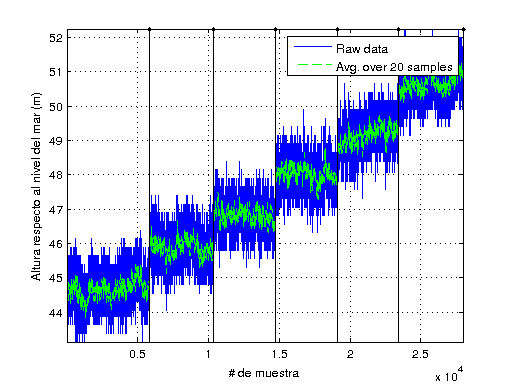
\includegraphics[width=0.34\textwidth]
		{./pics/esc1.png}}
	\subfloat[Segunda serie de medidas cada 1 metro]{\label{fig:esc2}
	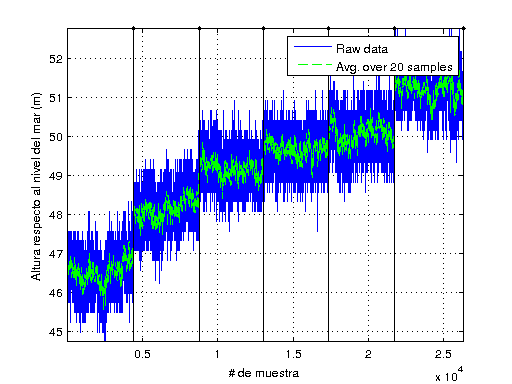
\includegraphics[width=0.34\textwidth]
		{./pics/esc2.png}}
	\subfloat[Medidas de altura subiendo y bajando]{\label{fig:variando}
	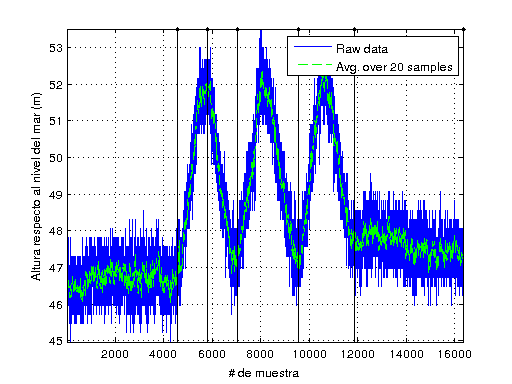
\includegraphics[width=0.34\textwidth]
		{./pics/variando.png}}		
  \end{center}
  \caption{Alturas obtenidas para medidas de alturas que distan un metro entre sí}
\end{figure}

En la tabla \ref{tab:alturasm} se muestran los valores de altura obtenidos en las distintas posiciones en las dos series de datos tomadas.

\begin{table}[H]
\centering
\begin{tabular}{c|c|c|} 

	  
	& \multicolumn{2}{|p{200pt}|}{\cellcolor[gray]{0.8} Altura medida con el barómetro (m)}      \\ \hline
\cellcolor[gray]{0.8} {Posición} & \cellcolor[gray]{0.8} {Serie 1} &\cellcolor[gray]{0.8} {Serie 2}\\ \hline

1 & 44.66 & 46.52 \\ \hline
2 & 45.87 & 48.12\\ \hline
3 & 46.82 & 49.15\\ \hline
4 & 48.04 & 49.66\\ \hline
5 & 49.15 & 50.05\\ \hline
6 & 50.66 & 51.21 \\ \hline
\end{tabular}
\caption{Alturas obtenidas con el barómetro}
\label{tab:alturasm}
\end{table}

Se observa inmediatamente en las medidas de altura realizadas que la altura absoluta registrada por el barómetro cambia considerablemente de una serie a la otra. En la segunda se observa que las medidas se encuentran en promedio un metro más arriba. Los puntos que se consideraron fueron los mismos, sin embargo las medidas fueron realizadas un día de tormenta. La presión atmosférica es muy cambiante en esos días. Eso puede explicar dicha diferencia. Asimismo, los datos que se presentan en la figura \ref{fig:variando} vienen a confirmar esa variación. Si bien el experimento comienza y termina a la misma altura, en la figura \ref{fig:variando} se observa que la altura medida es un metro superior al final del experimento respecto del principio.

Si bien las condiciones en las cuales se realizó el experimento no son las mejores nos permite extraer dos conclusiones importantes:

\begin{itemize}
\item Dada la variación de presión que puede haber en un día de tormenta no parece adecuado utilizar dicho instrumento como única fuente para conocer la altura del cuadricóptero en días donde la presión atmosférica sea susceptible de variaciones. 

\item El instrumento no sirve para determinar alturas absolutas. Si de un día a otro la presión cambia, también lo harán las alturas medidas. Esto implica que el barómetro de dos medidas de altura diferentes para el mismo punto. No se puede confiar en dicho instrumento para la medida absoluta de altura. 

\end{itemize}

En cuanto al error promedio y a la desviación estándar se obtuvo para las dos series:

\begin{itemize}
\item Serie 1:
		\begin{itemize}
		\item Error promedio: $-0.20m$
		\item Desviación estándar: $0.20m$
		\end{itemize}
\item Serie 2:
		\begin{itemize}
		\item Error promedio: $0.06m$
		\item Desviación estándar: $0.49m$
		\end{itemize}
\end{itemize}

Al tener pocas muestras en cada una de las series es imposible considerarlas como buenas muestras estadísticas, de hecho ambas difieren mucho en cuanto al error promedio que presentan y la desviación estándar. 

Si trabajamos con las dos series de datos lo que obtenemos es:

\begin{itemize}
\item Error promedio: $-0.07m$
\item Desviación estándar: $0.38m$
\end{itemize}



A partir de los datos anteriores se puede concluir que el $95.5 \%$ de las veces tendremos errores inferiores a $0.76m$ en diferencias de un metro. 
\subsubsection*{Medidas de altura que distan decenas de centímetros entre sí}

En la tabla \ref{tab:alturascm}


\begin{table}[H]
\centering
\begin{tabular}{|c|c|} 

	\cellcolor[gray]{0.8} {Altura medida con el barómetro(cm)} &
	\cellcolor[gray]{0.8} Altura medida con el metro (cm) \\ \hline
\end{tabular}
\caption{Alturas obtenidas con el metro y con el barómetro}
\label{tab:alturascm}
\end{table}


\end{document}